
\chapter{Whole-Body Controller on Visco Elastic Environment\label{chapter:wbc_visco_elastic}}

\graphicspath{{ChapterCompliantContact/figures}}

In Chapter~\ref{chapter:benchmarking_wbc}, we introduced a whole-body controller for humanoid robot locomotion in contact with a stiff environment. When the contact between a robot and its surroundings is sufficiently rigid, controllers based on the rigid contact assumption may nevertheless result in satisfactory robot performance. However, when contact compliance reduces robot performance, it is necessary to design contact models that account for contact stiffness and damping, which may subsequently be included in feedback controllers.
In light of that, this chapter presents a model of compliant contacts for time-critical humanoid robot motion control. The proposed model considers the environment as a continuum of spring-damper systems, allowing us to compute the equivalent contact force and torque that the environment exerts 
on the contact surface. We show that the proposed model extends the linear and rotational springs and dampers, classically used to characterize soft terrains,
to the case of \emph{large} contact surface orientations.
The contact model is then used for the 
real-time whole-body control of humanoid robots walking in visco-elastic environments. The overall approach is validated by simulating
walking motions of the iCub humanoid robot. Furthermore, we compare the proposed whole-body control strategy with state-of-the-art approaches. In this respect, we investigate the terrain compliance that makes the classical approaches that assumes rigid contacts fail. We finally analyze the robustness of the presented control design with respect to non-parametric uncertainty in the contact model.
\par
The chapter is organized as follows: Section~\ref{sec:contact_mode_compliant} presents the model used to characterize the interaction between the robot and the environment. Section~\ref{sec:controller_tsid_compliant} details the whole-body controller for walking on compliant surfaces. The section also contains the design of an observer to estimate the contact parameters. Section~\ref{sec:results_compliant} presents the simulation results on the iCub humanoid robot v2.7 -- see Section~\ref{sec:icub2.7}. Finally, Section~\ref{sec:conclusions_compliant} concludes the chapter.

The content of this chapter appears in:
\fciteWithVideoAndCode{Romualdi2021ModelingControl}{https://www.youtube.com/watch?v=7XKQ5ZWJvYU}{https://www.youtube.com/watch?v=7XKQ5ZWJvYU}{https://github.com/ami-iit/romualdi-2021-ral-soft\_terrain\_walking}{ami-iit/romualdi-2021-ral-soft\_terrain\_walking}

\section{Modeling of visco-elastic environments  \label{sec:contact_mode_compliant}}

Let us now consider a rigid body that makes a contact with a visco-elastic surface, and we assume that:
\begin{enumerate}
    \item there exists an inertial frame $\mathcal{I}$;
    \item there exist a frame $B$ rigidly attached to the body and we denote $o_B$ the origin of the frame and $[B]$ its orientation;
    \item all the point of the rigid body in contact with the environment define a set denoted with $\Omega \in \mathbb{R}^3$ and named \emph{contact domain}, we denote with ${}^B x$ a point on the contact surface expressed in the frame $B$, while with ${}^\mathcal{I} x$ the very same point expressed in the inertial frame $\mathcal{I}$;
    \item the environment characteristics are isotropic;
    \item the rigid body moves with a 6D velocity, denoted as ${}^{B[\mathcal{I}]} \mathrm{v}$ such that 
    \begin{equation}
    {}^{B[\mathcal{I}]} \mathrm{v} = 
    \begin{bmatrix}
       {}^\mathcal{I}\dot{o}_B \\
       {}^\mathcal{I}\omega_{\mathcal{I},B}
    \end{bmatrix} 
    \end{equation}
   where $B[\mathcal{I}] = \left(o_B, [\mathcal{I}]\right)$ is a frame having the origin in $o_B$ and oriented as $\mathcal{I}$.
    \item  $\forall x \in \Omega$, there exists a continuous pure force distribution that depends on the point ${}^\mathcal{I} x$ and its velocity ${}^\mathcal{I} \dot{x}$, i.e.,
    \begin{equation}
        \label{eq:compliant_model_rho_definition_subscript}
        \rho_x : \mathbb{R}^3 \times \mathbb{R}^3  \rightarrow \mathbb{R}^3.
    \end{equation}
\end{enumerate}
\begin{figure}[t]
    \centering
	\includegraphics{chapter_compliant_contact/figures/2d_contact.tikz}
	\caption[The visco-elastic model: a 2D representation.]{2D representation of the visco-elastic model. The gray rectangle represents the zero-force rigid body position. The orange rectangle is the body. $\Omega$ is the contact domain while $\bar{\mathcal{X}}$ is equal to $\Omega$ if the contact wrench is null ${}_{B[\mathcal{I}]} \mathrm{f} = 0$. The interaction between the rigid body and the environment can be approximate as a continuum of spring-damper systems. }
	\label{fig:2d_contact_model}
\end{figure}
Figure~\ref{fig:2d_contact_model} shows a rigid body in contact with a visco-elastic environment.

Each point of $\Omega$ may define a different function $\rho_x$. For the sake of simplicity, we assume that $\rho_x$ is the same for each point in contact with the environment. Consequently, we drop the subscript $x$ in Equation~\eqref{eq:compliant_model_rho_definition_subscript}. 
Given the above assumptions, the contact torque distribution about a point $o_B \in \mathbb{R}^3$, $\sigma_{o_B} : \mathbb{R}^3 \times \mathbb{R}^3  \rightarrow \mathbb{R}^3$ writes
    \begin{equation}
        \sigma_{o_B}\left({}^\mathcal{I}x, {}^\mathcal{I} \dot{x}\right) = \left({}^\mathcal{I}x - o_B\right)\times \rho\left({}^\mathcal{I}x, {}^\mathcal{I} \dot{x}\right).
    \end{equation}
Once the pure force and torque distribution are defined, then the equivalent contact 6D force expressed in mixed representation is given by \citep{Caron2015StabilityAreas} -- Section~\ref{sec:zmp}:
\begin{equation}
\label{eq:compliant-contact-contact-wrench}
    {}_{B[\mathcal{I}]} \mathrm{f} = \begin{bmatrix}
    {}_\mathcal{I} f \\
    {}_{B[\mathcal{I}]} \mu
    \end{bmatrix} = 
    \begin{bmatrix}
    \int_\Omega \rho \diff \Omega \\
    \int_\Omega \sigma_{o_B} \diff \Omega \\
    \end{bmatrix}.
\end{equation}
\par
We now propose a model that can be used to describe the contact between a body and a compliant environment.
\begin{lemma}
\label{lemma:compliant_model}
Let $\bar{\mathcal{X}}$ the set of points $\bar{x}\in\mathbb{R}^3$:
\begin{equation}
     \bar{\mathcal{X}} = \{ \bar{x}\in\mathbb{R}^3  : \rho(\bar{x}, 0) = 0  \}.
\end{equation}
Assume that: $i)$ the contact domain $\Omega$ is a rectangle of dimensions $l$ and $w$; $ii)$ the point $o_B {\in} \mathbb{R}^3$ is the center of the rectangular domain;  $iii)$ the distribution $\rho$ is given by:
\begin{equation}
\rho\left({}^\mathcal{I} x, {}^\mathcal{I} \dot{x}\right) = k \left( {}^\mathcal{I} \bar{x} - {}^\mathcal{I} x\right) - b \; {}^\mathcal{I} \dot{x},
\label{eq:contact_model_general}
\end{equation}
with $k>0$ and $b>0$.
\par
Then, the equivalent contact force and torque $ {}_{B[\mathcal{I}]} \mathrm{f}$ \eqref{eq:compliant-contact-contact-wrench} are given by
\begin{IEEEeqnarray}{rcl}
\phantomsection \label{eq:contact_wrench_integral_rectangle}
 \IEEEyesnumber  \IEEEyessubnumber*
\label{eq:contact_force_integral_rectangle}
{}_\mathcal{I} f  &\;=\;& lw |e _ 3^\top \prescript{\mathcal{I}}{}R _B e _ 3| [k (\bar{o}_B - o_B) - b \dot{o}_B] \\
\label{eq:contact_torque_integral_rectangle}
{}_{B[\mathcal{I}]} \mu &=&  \frac{l w}{12} |e _ 3^\top \prescript{\mathcal{I}}{}{R} _B e _ 3| \nonumber \\
&&\left\{l^2  (\prescript{\mathcal{I}}{}{R} _B e_1) \times [b  (\prescript{\mathcal{I}}{}{R} _B e_1) \times {}^{\mathcal{I}} \omega _ {\mathcal{I},B} + k   \prescript{\mathcal{I}}{}{\bar{R}} _B e_1]  \right .  \\
&& + \left . w^2  (\prescript{\mathcal{I}}{}{R} _B e_2) \times [b  (\prescript{\mathcal{I}}{}{R} _B e_2) \times {}^{\mathcal{I}} \omega _ {\mathcal{I},B} + k   \prescript{\mathcal{I}}{}{\bar{R}} _B e_2] \right\} \nonumber,
\end{IEEEeqnarray}
where $\prescript{\mathcal{I}}{}R _B$ is the rotation from the inertial frame $\mathcal{I}$ to a frame rigidly attached to the body $B$.
$\dot{o}_B$ and ${}^{\mathcal{I}} \omega _ {\mathcal{I}, B}$ are the linear and angular velocity of the rigid body expressed in mixed representation. $\bar{o}_B$ and  $\prescript{\mathcal{I}}{}{\bar{R}} _{B}$ are the position and the rotation of the frame $B$ such that in case of zero velocity, the 6D force is null. 
\end{lemma}
The set $\bar{\mathcal{X}}$ can also be defined by considering a point $P$ that belongs to the contact domain $\Omega$ of the rigid body $B$ in contact with the compressible environment. Then, the point $P$ can move to a point $P_0$ of the space such that the force distribution at the point $P_0$ is zero. In coordinates, let $P$ be defined by the coordinate vector $x_p \in \mathbb{R}^3$ and $P_0$ be defined by the coordinate vector $\bar{x}_p \in \mathbb{R}^3$. Then given $x_p$
\begin{equation}
    \rho(\bar{x}_p, 0) = 0.
\end{equation}
$\bar{\mathcal{X}}$ contains all the points $\bar{x}_p$ associated with each point $P$ belonging to the contact domain $\Omega$.
\begin{figure}[t]
\centering
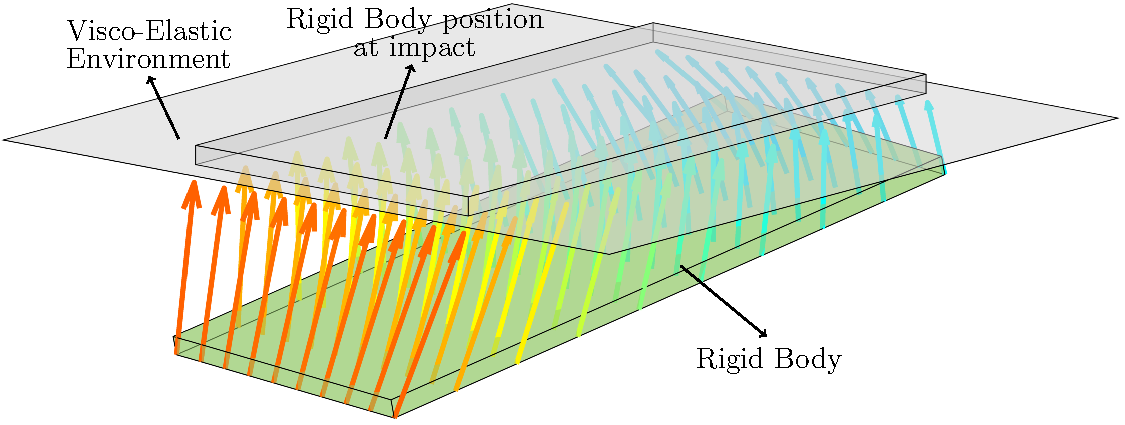
\includegraphics[width=1\columnwidth]{chapter_compliant_contact/figures/paper_fig.pdf}
\caption[Vector field generated by the visco-elastic model]{Vector field generated by the visco-elastic model -- Equation~\eqref{eq:contact_model_general}. The grey box represents the zero-force rigid-body position. The green parallelepiped is the body. The arrows represent the forces that act on the contact surface; the lighter the color, the higher the force magnitude. \label{fig:contact_model_vector_field}}
\end{figure}
The proof of Lemma~\ref{lemma:compliant_model} is in Appendix~\ref{appendix:proof_lemma_compliant}.
\par
Lemma~\ref{lemma:compliant_model} shows that the 6D contact force \eqref{eq:compliant-contact-contact-wrench} depends only on the distribution of the contact force $\rho$ on the shape of the contact domain $\Omega$ and on the rigid body state, namely \emph{position}, \emph{orientation}, \emph{linear} and \emph{angular velocity}. As a consequence, we avoid using rotational springs and dampers to describe the interaction between the robot and the environment. Furthermore, Lemma~\ref{lemma:compliant_model} also contains a close solution for the equivalent contact wrench \eqref{eq:contact_force_integral_rectangle} \eqref{eq:contact_torque_integral_rectangle} in the case of a linear contact model~\eqref{eq:contact_model_general} and a rectangular contact surface $\Omega$. As a consequence, it can be exploited in hard-real-time applications such as control architectures.
To give the reader a better understanding, we can imagine that the set $\bar{\mathcal{X}}$ contains the position of all the points on the foot sole at the touch down. Once the contact is established, the environment is deformed. The interaction between the foot and the environment is then approximated as a continuum of spring-damper systems -- Equation~\eqref{eq:contact_model_general}.
Each spring-damper system exerts a force on the associated point of the contact domain. Combining all forces, we can imagine that the rigid body is subject to the vector field represented in Figure~\ref{fig:contact_model_vector_field}. 
Finally, we want to recall that, since the contacts are unilateral, this model is valid as long as the normal forces are positive and the tangential component lies inside the friction cone.

\subsection{Linear approximation of the visco-elastic model}
It is worth noting that the model~\eqref{eq:contact_force_integral_rectangle}-\eqref{eq:contact_torque_integral_rectangle} also encompasses the classical linear modeling techniques for soft terrains. The following corollary shows, in fact, that linear approximations of~\eqref{eq:contact_force_integral_rectangle}-\eqref{eq:contact_torque_integral_rectangle} lead to linear and rotational springs and dampers that are usually used to model contact wrenches due to soft terrains~\cite[Equation~(8)]{Sygulla2020AFootholds:}.
\begin{corollary}
\label{corollary:approximation}
Let ${}_{\mathcal{I}} f$ and ${}_{B[\mathcal{I}]} \mu $ be the contact force and torque given by \eqref{eq:contact_force_integral_rectangle} and \eqref{eq:contact_torque_integral_rectangle}, respectively. Assume that $\prescript{\mathcal{I}}{}{\bar{R}} _B = I _3 $ and $\prescript{\mathcal{I}}{}{R} _B$ is approximated with its first order of the Taylor expansion, i.e., $\prescript{\mathcal{I}}{}R _B = I_3 + \Theta\times$, with $\Theta \in \mathbb{R}^3$. Assume that $\Theta$ represents the classical sequence of roll-pitch-yaw, namely $\prescript{\mathcal{I}}{}R _B(\Theta) = R_z(\Theta_3)R_y(\Theta_2)R_x(\Theta_1)$.
Then, the contact model \eqref{eq:contact_force_integral_rectangle}-\eqref{eq:contact_torque_integral_rectangle} writes 
\begin{IEEEeqnarray}{c}
\phantomsection \label{eq:linear_model}
 \IEEEyesnumber  \IEEEyessubnumber*
    {}_{\mathcal{I}} f_l = \mathcal{K}_l (\bar{o}_B - o_B) - \mathcal{B}_l \dot{o}_B, \label{eq:linear_model_force}\\ 
    {}_{B[\mathcal{I}]} \mu_l = - \mathcal{K}_a \Theta - \mathcal{B}_a \dot{\Theta} \IEEEyessubnumber* \label{eq:linear_model_torque},
\end{IEEEeqnarray}
with 
\begin{equation}
\mathcal{K}_l = l w k I_3, \quad \mathcal{K}_a =  k \frac{l w}{12} \begin{bmatrix} w ^ 2 & 0 & 0 \\ 
0 & l ^ 2 & 0 \\ 
0 & 0& l ^2 {+} w ^2 \end{bmatrix}
\end{equation}
\begin{equation}
\mathcal{B}_l = l w b I_3, \quad \mathcal{B}_a =  b \frac{l w}{12} \begin{bmatrix} w ^ 2 & 0 & 0 \\ 
0 & l ^ 2 & 0 \\ 
0 & 0& l ^2 {+} w ^2 \end{bmatrix}
\end{equation}
\end{corollary}

The proof of Corollary~\ref{corollary:approximation} is in Appendix~\ref{appendix:proof_corollary_compliant}.
Corollary~\ref{corollary:approximation} thus shows that
the model~\eqref{eq:contact_force_integral_rectangle}-\eqref{eq:contact_torque_integral_rectangle} extends the linear models~\citep{Sygulla2020AFootholds:} to the case of \emph{large} contact surface orientations. 
\par
Here, we want to underline that the classical linear approaches for modeling compliant contacts ~\eqref{eq:linear_model} -- for example, rotational springs and dampers \citep{Sygulla2020AFootholds:}~-- are often valid only for \emph{small} contact surface rotations. This is due to the minimal representation (i.e., three angles, such as \emph{roll}, \emph{pitch}, \emph{yaw}) used to represent $\SO(3)$. In addition, the equivalent \emph{rotational stiffness and dampers} values $\mathcal{K}_a$ and $\mathcal{B}_a$ are often not related to the physical parameters of the contact. On the other hand, even if the model we propose ~\eqref{eq:contact_force_integral_rectangle}-\eqref{eq:contact_torque_integral_rectangle} is indeed a 6d force, it is obtained by integrating pressure and shear stresses distributions to better catch the fundamental effects of the contact physics, without having the aforementioned issues of classical rotational spring and damper models.
\par
\begin{figure}[t]
\centering
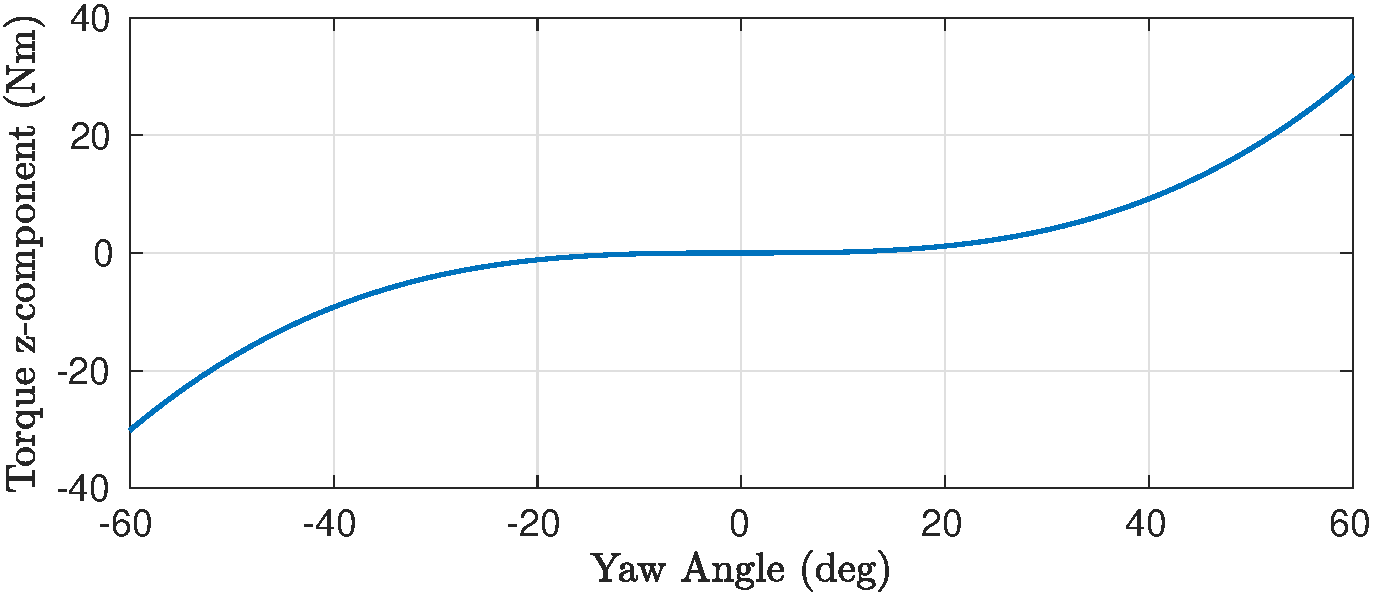
\includegraphics[width=0.9\columnwidth]{chapter_compliant_contact/figures/comparison_lumped_continuous.pdf}
\caption{Linear approximation error for different values of yaw angle.
\label{fig:approximation_error}}
\end{figure}
Let us now introduce the approximation error between the linear model~\eqref{eq:linear_model} and the model presented~\eqref{eq:contact_wrench_integral_rectangle} as $\epsilon_\mathrm{f} = {}_{B[\mathcal{I}]} \mathrm{f}  - {}_{B[\mathcal{I}]}\mathrm{f}_l$.
Figure~\ref{fig:approximation_error} shows the last component of the error $\epsilon_\mathrm{f}$, i.e., $e_6^\top \epsilon_\mathrm{f}$, in the case of zero velocity and zero pitch and roll angles. The higher the angle, the greater the difference. Thus, the higher is the angle, the less valid the linear approximation is. A similar analysis holds also for the other components of the 6D force. 
To conclude, the model presented in Lemma~\ref{lemma:compliant_model} is not equivalent to a linear lumped contact model, but it can be seen as a non-linear generalization while keeping a low mathematical complexity.



    












\section{Whole-body controller \label{sec:controller_tsid_compliant}}

The whole-body controller aims to track kinematic and dynamic quantities.
The proposed whole-body controller computes the desired joint torques using the robot joint dynamics~\eqref{eq:robot_dynamics_joints}, where the robot acceleration $\dot{\nu}$ is set to the desired \emph{starred} quantity and the contact wrenches ${}_{\mathcal{C}_k[\mathcal{I}]}\mathrm{f}_k$ are estimated or measured:
\begin{equation}
    \label{eq:forward_dynamics_compliant}
    \tau^* = M_{s}(q) \dot{\nu}^* + h_{s} (q, \nu) - \sum_{k = 1}^{n_c} J^\top_{{\mathcal{C}_k}_s}(q)  \; {}_{\mathcal{C}_k[\mathcal{I}]}\mathrm{f}_k.
\end{equation}
The desired generalized robot acceleration $\dot{\nu}^{*}$ is chosen to follow the desired centroidal momentum trajectory, the torso and root orientation, and the feet pose, while considering the contact model presented in Section~\ref{sec:contact_mode_compliant}.
\par 
The control problem is formulated using the stack of tasks approach. The control objective is achieved by framing the controller as a constrained optimization problem where the low priority tasks are embedded in the cost function, while the high priority tasks are treated as constraints.

\subsection{Low and high priority tasks \label{sec:tsid_compliant_tasks}}
What follows presents the tasks required to evaluate the desired generalized robot acceleration $\dot{\nu}^{*}$. 
\subsubsection{Centroidal momentum task}
In case of visco-elastic contacts, the contact wrench ${}_{\mathcal{C}_k[\mathcal{I}]}\mathrm{f}_k$ cannot be arbitrarily chosen. From now on, we assume that we can control the contact wrench derivative ${}_{\mathcal{C}_k[\mathcal{I}]}\dot{\mathrm{f}}_k$. Thus, by differentiating the centroidal momentum dynamics~\eqref{eq:centroidal_momentum_dynamics}, we obtain:


\begin{equation}
    \label{eq:centroidal_momentum_derivative}
    {}_{\bar{G}} \ddot{h} = \sum_{k = 1}^{n_c} \begin{bmatrix}
  0_{3\times3} & 0_{3\times3} \\
  \left({}^{\mathcal{I}}\dot{p}_k - \dot{x}_\text{CoM}\right)\times & 0_{3\times3}
  \end{bmatrix} {}_{\mathcal{C}_k[\mathcal{I}]}\mathrm{f}_k + \begin{bmatrix}
	I_3 & {0}_{3\times 3} \\
	\left({}^{\mathcal{I}}{p}_k - {x}_\text{CoM}\right)\times & I_3 
	\end{bmatrix} {}_{\mathcal{C}_k[\mathcal{I}]}\dot{\mathrm{f}}_k
\end{equation}
To follow the desired centroidal momentum trajectory, we minimize the weighted norm of the error between the robot centroidal momentum and the desired trajectory:
\begin{equation}
    \Psi_h = \frac{1}{2} \norm{{}_{\bar{G}} \ddot{h} ^ * -{}_{\bar{G}} \ddot{h}}_{\Lambda_h},
\end{equation}
where $\Lambda _ h$ is a positive definite diagonal matrix. ${}_{\mathcal{C}_k[\mathcal{I}]}\mathrm{f}_k$ is the estimated/measured contact wrench. ${}_{\bar{G}}\ddot{h}^*$ is the desired centroidal momentum derivative, and it is responsible for stabilizing the desired centroidal momentum dynamics:

\begin{equation}
\begin{split}
    {}_{\bar{G}}\ddot{h}^* &= {}_{\bar{G}}\ddot{h}^\text{ref} + k_h^d ({}_{\bar{G}}\dot{h}^\text{ref} - {}_{\bar{G}}\dot{h}) + k_h^p ({}_{\bar{G}} h^\text{ref} - {}_{\bar{G}} h) \\ 
    &+ k_h^i \int {}_{\bar{G}} h^\text{ref} - {}_{\bar{G}} h \diff t,
    \end{split}
\end{equation}
where the integral of the angular momentum is computed numerically.
Here, $k^d_h$, $k^p_h$, and $k^i_h$ are three diagonal matrices. When the equality holds, the centroidal dynamics converges exponentially to the reference value if and only if $k^p_h$, $k^i_h$ and $k_h^d k_h^p -k_h^i$ are positive definite.  

\subsubsection{Torso and root orientation tasks}
While walking, we require the torso and the root frames to have a specific orientation with respect to the inertial frame. To accomplish this task, we minimize the norm of the error between a desired angular acceleration and the actual frame angular acceleration:
\begin{equation}
    \Psi_\circ = \frac{1}{2} \norm{\dot{\omega}_\circ ^ {*} - (\dot{J} _{\circ} \nu + J _{\circ} \dot{\nu})}^2  _ {\Lambda _ \circ},
\end{equation}
where the subscript $\circ$ indicates the frames of root $R$ and torso $T$. $\Lambda _ \circ$ is a positive definite matrix that weighs the contributions in different directions. $\dot{\omega} ^*_\circ$ is set to guarantee almost global stability and convergence of $\prescript{\mathcal{I}}{}{R}_{\circ}$ to $ \prescript{\mathcal{I}}{}{R}_{\circ} ^\text{ref}$ \citep{Olfati-Saber:2001:NCU:935467}:

\begin{IEEEeqnarray}{LL}
\IEEEyesnumber
\dot{\omega}^{*}_\circ &= \dot{\omega}^\text{ref} - c_0 \left(\hat{\omega} \prescript{\mathcal{I}}{}{R}_{\circ} \prescript{\mathcal{I}}{}{R}_{\circ} ^{\text{ref} ^ \top} - \prescript{\mathcal{I}}{}{R}_{\circ} \prescript{\mathcal{I}}{}{R}_{\circ} ^{\text{ref}^{\top}} \hat{\omega}^\text{ref}\right)^{\vee} \nonumber\\
&- c_1 \left(\omega - \omega^\text{ref}\right) - c_2 \left(\prescript{\mathcal{I}}{}{R}_{\circ} \prescript{\mathcal{I}}{}{R}_{\circ} ^{\text{ref}^{\top}}\right) ^\vee. \label{eq:rotational_pid_acceleration}
\end{IEEEeqnarray}

Here, $c_0$, $c_1$, and $c_2$ are positive numbers.

\subsubsection{Swing foot task}
Concerning the tracking of the swing foot trajectory, we minimize the following cost function
\begin{equation}
    \Psi_{F} = \frac{1}{2} \norm{\dot{\mathrm{v}}_{F} ^ {*} - (\dot{J} _{F} \nu + J _{F} \dot{\nu})}^2 _ {\Lambda _ {F}},
\end{equation}
the angular part of $\dot{\mathrm{v}}^{*}_{F}$ is given by \eqref{eq:rotational_pid_acceleration} where the subscript $\circ$ is replaced by $F$, while the linear part $\ddot{p}^{*}$ is equal to $\ddot{p}^{*}_{F} =  \ddot{p}\,^\text{ref}_{F} - k^d _{x _{f}} (\dot{p}_{F} - \dot{p}^\text{ref}_{F}) - k^p _{x _{f}} (p_{F} - p^\text{ref}_{F})$.
Here, the gains are again positive definite matrices.

\subsubsection{Regularization tasks}
In order to prevent the controller from providing solutions with huge joint variations, we introduce a regularization task for the joint variables. The task is achieved by asking for a desired joint acceleration that depends on the error between the desired and measured joint values, namely:
\begin{equation}
    \Psi_s = \frac{1}{2} \norm{k_s^p(s^\text{ref} -s) - k_s^d \dot{s} - \ddot{s}}^2  _ {\Lambda _ s},
\end{equation}
where $s^\text{ref}$ is a desired joint configuration, $k_s^d$, $k_s^p$ and $\Lambda _ s$ are symmetric positive definite matrices. 
To reduce the amount of the contact wrench required to accomplished the centroidal momentum tracking, the following task is considered:
\begin{equation}
    \Psi_{\mathrm{f}_k} = \frac{1}{2} \norm{k_f^p\left({}_{\mathcal{C}_k[\mathcal{I}]}\mathrm{f}_k^\text{ref} -{}_{\mathcal{C}_k[\mathcal{I}]}\mathrm{f}_k\right) - {}_{\mathcal{C}_k[\mathcal{I}]}\dot{\mathrm{f}}_k}^2  _ {\Lambda _ {f_k}}.
\end{equation}
Here, $\Lambda _ {f_k}$ and $k_f^p$ are positive definite matrices. ${}_{\mathcal{C}_k[\mathcal{I}]}\mathrm{f}_k$ is the estimated/measured contact wrench and ${}_{\mathcal{C}_k[\mathcal{I}]}\mathrm{f}^\text{ref}_k$ is the desired force regularization value.
\subsubsection{Contact wrench feasibility}
The feasibility of the contact wrenches ${}_{\mathcal{C}_k[\mathcal{I}]}\mathrm{f}_k$ is generally guaranteed by another set of inequalities of the form:
\begin{equation}
    \label{eq:contact_wrench_feasibility_constraint}
    A_{\mathcal{C}_k[\mathcal{I}]} \; {}_{\mathcal{C}_k[\mathcal{I}]}\mathrm{f}_k \le b.
\end{equation}
where $A_{\mathcal{C}_k[\mathcal{I}]}$ is a matrix that depends on the position of the robot joints and the base pose.
\par
More specifically, ${}_{\mathcal{C}_k[\mathcal{I}]}\mathrm{f}_k$ must belong to the associated friction cone, while the position of the local CoP is restricted within the support polygon. However, in the case of visco-elastic contacts, the contact wrenches cannot be arbitrarily chosen. This limitation can be overcome by discretizing the contact wrench dynamics using the forward Euler method:
\begin{equation}
    \label{eq:contact_force_discerization}
    {}_{\mathcal{C}_k[\mathcal{I}]}\mathrm{f}_k^{i+1} = {}_{\mathcal{C}_k[\mathcal{I}]}\mathrm{f}_k^{i} + {}_{\mathcal{C}_k[\mathcal{I}]}\dot{\mathrm{f}}_k^i \diff t,
\end{equation}
where $T$ is the constant integration time. 
We can require the contact wrench at the next instant to guarantee the inequality constraints \eqref{eq:contact_wrench_feasibility_constraint}.
Combining \eqref{eq:contact_force_discerization} and \eqref{eq:contact_wrench_feasibility_constraint}, we can now obtain a tractable set of inequality constraints
\begin{equation}
A_{\mathcal{C}_k[\mathcal{I}]}\; {}_{\mathcal{C}_k[\mathcal{I}]}\dot{\mathrm{f}}_k \diff t  \le b -  A  {}_{\mathcal{C}_k[\mathcal{I}]}\mathrm{f}_k,    
\end{equation}
 
where the superscript $i$ has been dropped, and ${}_{\mathcal{C}_k[\mathcal{I}]}\mathrm{f}_k$ represents the measured/estimated contact wrench.
\subsubsection{Floating-base system base dynamics}
The whole-body controller considers the base system dynamics presented in Equation~ \eqref{eq:robot_dynamics_base} as:
\begin{equation}
    \label{eq:base_dynamics_compliant}
    M_\nu \dot{\nu} + h_\nu = \sum_{k = 1}^{n_c} J^\top_{\mathcal{C}_k} {}_{\mathcal{C}_k[\mathcal{I}]}{\mathrm{f}}_k.
\end{equation}
where ${}_{\mathcal{C}_k[\mathcal{I}]}\mathrm{f}_k$ are the measured/estimated contact wrenches. 
\subsubsection{Contact model dynamics}
The contact wrench dynamics can be obtained by differentiating equations \eqref{eq:contact_force_integral_rectangle} and \eqref{eq:contact_torque_integral_rectangle}. 
By computing the time derivative of $f$, one has the following control-affine dynamical system:
\begin{equation}
    \label{eq:force_derivative_affine_system}
    {}_{\mathcal{C}_k[\mathcal{I}]}\dot{\mathrm{f}}_k  =  h_{\mathrm{f}_k} + g_{\mathrm{f}_k} {}^{\mathcal{C}_k[\mathcal{I}]}\dot{\mathrm{v}}_{F_k}
\end{equation}
where $h_{\mathrm{f}_k} \in \mathbb{R}^6$ and $g_{\mathrm{f}_k}\in\mathbb{R}^{6 \times 6}$ is full rank for each possible admissible state. By explicating the dependence on the robot generalized acceleration, Equation~\eqref{eq:force_derivative_affine_system} writes as:
\begin{equation}
 \label{eq:contact_wrench_dynamics_qp}
 {}_{\mathcal{C}_k[\mathcal{I}]}\dot{\mathrm{f}}_k  =  h_{\mathrm{f}_k} + g_{\mathrm{f}_k} \left(J_{F_k}(q) \dot{\nu} + \dot{J}_{F_k}(q) \nu \right).
\end{equation}

\subsection{Quadratic programming problem \label{sec:tsid_flex_optimal_control_problem}}
The control objective is achieved by casting the control problem as a constrained optimization problem whose conditional variables are $\dot{\nu}$ and $\dot{f}_k$ where $k$ represents the foot in contact with the environment, namely left, right, or both.
In details:
\begin{IEEEeqnarray}{CCL}
\phantomsection \label{eq:acceleration_QP}  \IEEEyesnumber  \IEEEyessubnumber*
\minimize\limits_{\dot{\nu},  \dot{f}_k}  && \Psi_h + \Psi_\mathcal{T} + \Psi_\mathcal{R} + \Psi_F + \Psi_s + \Psi_{\mathrm{f}_k} \\
\text{subject to}& \quad & A_{\mathcal{C}_k[\mathcal{I}]}\; {}_{C_k[\mathcal{I}]} \dot{\mathrm{f}}_k \diff T \le b -  A_{\mathcal{C}_k[\mathcal{I}]} \; {}_{C_k[\mathcal{I}]} \mathrm{f}_k \\
&& M_\nu \dot{\nu} + h_\nu = \sum_{k = 1}^{n_c} J^\top_{\mathcal{C}_k} {}_{\mathcal{C}_k[\mathcal{I}]} \mathrm{f}_k  \\
&&  {}_{\mathcal{C}_k[\mathcal{I}]}\dot{\mathrm{f}}_k  =  h_{\mathrm{f}_k} + g_{\mathrm{f}_k} \left(J_{F_k}(q) \dot{\nu} + \dot{J}_{F_k}(q) \nu \right). 
\end{IEEEeqnarray}
We notice that the system base dynamics~\eqref{eq:base_dynamics_compliant} and the contact dynamics~\eqref{eq:contact_wrench_dynamics_qp} depend linearly on the decision variables $\dot{\nu}$ and ${}_{C_k[\mathcal{I}]} \mathrm{f}_k$. Furthermore, the tasks presented in Section~\ref{sec:tsid_compliant_tasks} depend quadratically on the decision variables. Consequently, the optimization problem in~\eqref{eq:acceleration_QP} can be transcribed into a quadratic programming problem (see Section~\ref{sec:qp}) and solved via off-the-shelf solvers. Once the desired robot acceleration $\dot{\nu}^*$ is computed, the desired joint torques can be easily evaluated with Equation~\eqref{eq:forward_dynamics_compliant}.

\begin{figure}[t]
\centering
\includegraphics{chapter_compliant_contact/figures/block_diagram.tikz}
\caption{Controller architecture.}\label{fig:block-diagram-compliant}
\end{figure}

\subsection{Contact parameters estimation}
The optimal control problem presented in Section~\ref{sec:tsid_compliant_tasks} is based on the perfect knowledge of the contact parameters $k$ and $b$. In a simulated environment, the value of the parameters is perfectly known. However, in the real scenario, an estimation algorithm is required to compute the parameters.
\par
The contact model described by Equations \eqref{eq:contact_force_integral_rectangle} and \eqref{eq:contact_torque_integral_rectangle} is linear with respect to the contact parameters as $ {}_{B[\mathcal{I}]} \mathrm{f}  = \mathcal{Y}(o_B, \prescript{\mathcal{I}}{} R _ B, \dot{o}_B, \prescript{\mathcal{I}}{} \omega _ {\mathcal{I}, B}) \pi$,
where $\mathcal{Y}(o_B, \prescript{\mathcal{I}}{} R _ B, \dot{o}_B, \prescript{\mathcal{I}}{} \omega _ {\mathcal{I}, B})  \in \mathbb{R} ^{6 \times 2}$ is the regressor and is equal to 



\begin{equation}
\mathcal{Y} = lw |e _ 3^\top R e _ 3| 
\begin{bmatrix}
\bar{o}_B - o_B & - \dot{o}_B \\
\frac{l^2}{12}\left((R e_1) \times\right) \bar{R} e_1 + \frac{w^2}{12} \left((R e_2) \times\right) \bar{R} e_2 &   \left[\frac{l^2}{12} \left((R e_1) \times\right)^2  + \frac{w^2}{12} \left((R e_2) \times\right) ^2 \right]\omega
\end{bmatrix}
\end{equation}
where, for sake of clarity, we removed all the prefixes and suffices. 
$\pi \in \mathbb{R}^2$ contains the spring and damper coefficients, i.e.,
\begin{equation}
\pi = \begin{bmatrix} k \\ b \end{bmatrix}.
\end{equation}
We aim to estimate the contact parameters $\hat{\pi}$ so that the \emph{least-squares} criterion is minimized. Namely, we seek for $\hat{\pi}$ such that the error between the measured contact forces and the predicted contact force is minimized over a time windows having a length of $t$ samples: 
\begin{equation}
    \label{eq:rls_definition}
    \hat{\pi}_t = \argmin\limits_{\pi} \frac{1}{2} \sum_{i=1}^t\norm{{}_{B[\mathcal{I}]} \mathrm{f}[i]- \mathcal{Y}_i \pi}^2 _{\Gamma_i}.
\end{equation}
Here, $\Gamma _i \succ 0$ is a strictly positive definite matrix. ${}_{B[\mathcal{I}]} \mathrm{f}[i]$ and $\mathcal{Y}_i$ represent the forces and the regressor computed at instant $i$. 
\par
We solved this problem by applying the Recursive least squares (RLS) filter \citep[Section~11.2]{Ljung1999} as:
\begin{equation}
    \label{eq:contact_param_est}
    \hat{\pi}_t = \hat{\pi}_{t-1} + L_t \left[{}_{B[\mathcal{I}]} \mathrm{f}[t] - \mathcal{Y}_t \hat{\pi}_{t-1}\right],
\end{equation}
where ${}_{B[\mathcal{I}]} \mathrm{f}[t] - \mathcal{Y}_t \hat{\pi}_{t-1}$ is the innovation at time $t$. The gain $L_t \in \mathbb{R}^{2\times6}$ is given by:
\begin{equation}
    \label{eq:kalman}
    L_t = P_{t-1} \mathcal{Y}_t^\top \left[ \Gamma_t + \mathcal{Y}_t P_{t-1} \mathcal{Y}_t^\top\right]^{-1},
\end{equation}
$P_{t-1}$ is the estimation error covariance at the instant $t-1$:
\begin{equation}
    \label{eq:contact_param_cov}
    P_t = \left[I_ 2- L_t \mathcal{Y}_t\right] P_{t-1} \left[I_2 - L_t \mathcal{Y}_t\right]^\top + L_t \Gamma_t  L_t^\top.
\end{equation}
\par
At every time step, Equations \eqref{eq:contact_param_est}-\eqref{eq:kalman}-\eqref{eq:contact_param_cov} are used to estimate the contact parameters $k$ and $b$. 
\par
In the case of zero linear and angular velocity, the last three columns of $\mathcal{Y}$ are zero, so the damper parameter is not observable when the contact surface does not move. Walking simulations we performed tend to show that the foot velocity is almost always different from zero when in contact with the ground. So, the contact parameters are, in practice, observable during robot walking.
\par
Equations \eqref{eq:contact_param_est}-\eqref{eq:kalman}-\eqref{eq:contact_param_cov} are historically derived from the recursive least square theory~\citep[Section~ 9.3]{Hayes1996StatisticalModeling} and \citep[Section~11.2]{Ljung1999}. However, we notice that the very same results can be obtained by designing a Kalman filter~\citep{Kalman1960AProblems}\footnote{Considering a Linear Time Invariant discrete (LTI) dynamical system of the form
\begin{IEEEeqnarray*}{l}
x_{k+1}  = F x_k + G u_k + w_k\\
z_k = H x_k + v_k
\end{IEEEeqnarray*}
where $x_k$ is the state of the system, $u_k$ is the exogenous input, $z_k$ is the measurement vector. $w_k$ is the process noise vector that is assumed to be zero-mean Gaussian with covariance $Q$, i.e.,, $w_k \sim \mathcal{N}(0, Q)$. $v_k$ is the measurement noise vector. It is assumed to be zero-mean Gaussian with covariance $R$, i.e.,, $v_k \sim \mathcal{N}(0, R)$. The Kalman filter~\citep{Kalman1960AProblems} is a recursive algorithm that estimates the state $x_k$ starting from a series of measurements. It is possible to prove that the Kalman filter is the optimal observer in the case of linear dynamics and Gaussian noises $w_k$ and $v_k$.} considering the following dynamical system
\begin{equation}
    \pi_{t+1} = \pi_t,
\end{equation}
having as a measurement equation
\begin{equation}
    {}_{B[\mathcal{I}]} \mathrm{f}[t] =  \mathcal{Y}_t \pi_t + \psi_t,
\end{equation}
where $\psi$ is a white Gaussian noise having zero mean and covariance $\mathrm{E}\left[\psi_t \psi_t^\top\right] = \Gamma_t$.


\begin{figure}[t]
        \begin{subfigure}[b]{0.32\textwidth}
        \centering
        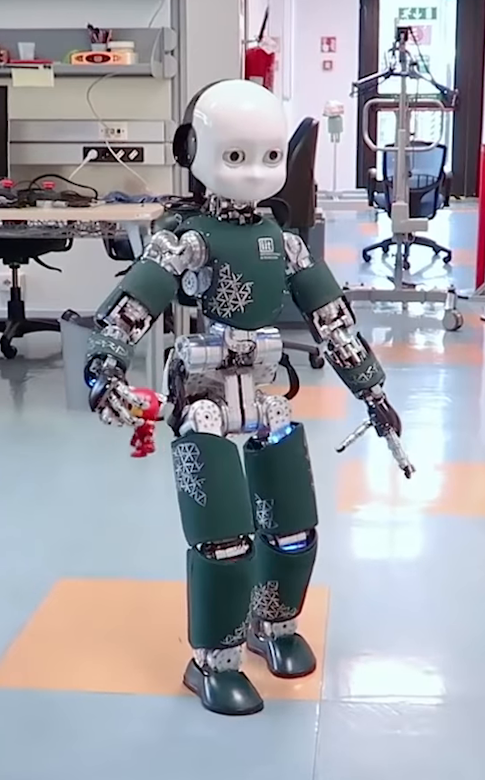
\includegraphics[width=\columnwidth]{chapter_simplified_benchmarking/figures/step1.png}
    \end{subfigure}
    \hfill
           \begin{subfigure}[b]{0.32\textwidth}
        \centering
        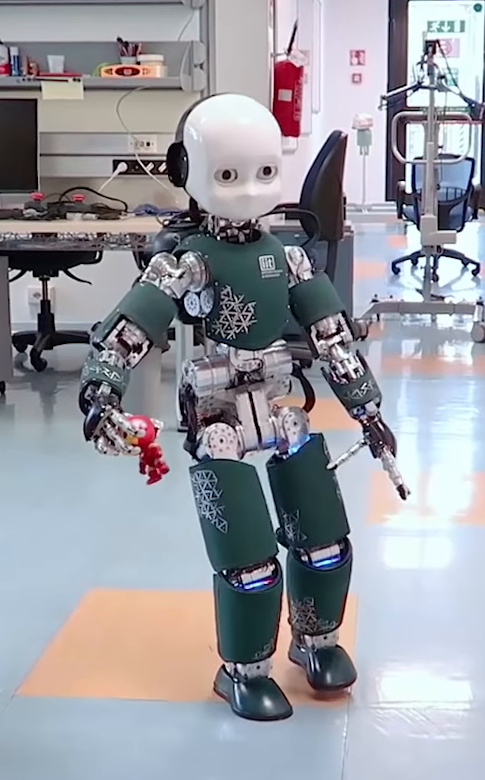
\includegraphics[width=\columnwidth]{chapter_simplified_benchmarking/figures/step2.png}
    \end{subfigure}
    \hfill
           \begin{subfigure}[b]{0.32\textwidth}
        \centering
        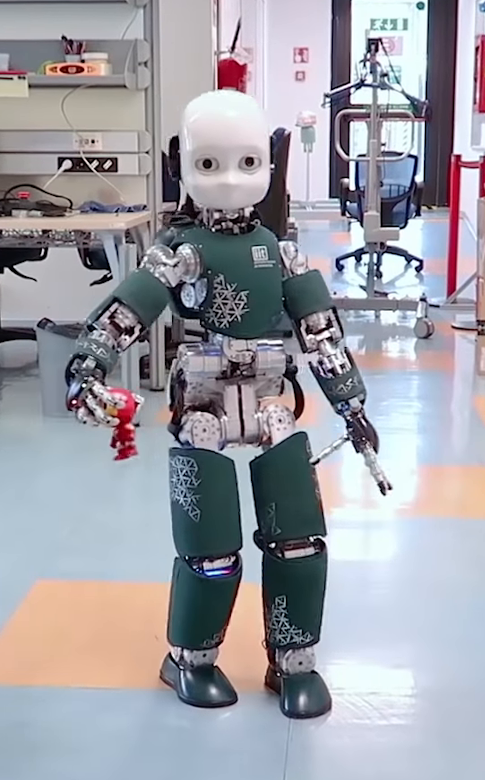
\includegraphics[width=\columnwidth]{chapter_simplified_benchmarking/figures/step3.png}
    \end{subfigure}
    \caption{The iCub robot walks with the 3 layer controller architecture of Figure~\ref{fig:three-layer-simplified-benchmarking}.}
    \label{fig:icub_walking_simplified}
\end{figure}

\section{Results}
\label{sec:results_simplified_benchmarking}
In this section, we present experiments obtained with several implementations of the simplified model controllers, namely: the \emph{instantaneous} and the \emph{predictive} controllers.

To benchmark the different simplified model controllers, we test the algorithms on the iCub humanoid robot v2.7 -- Section~\ref{sec:icub2.7}. We attach the simplified control layer to the three-layer controller architecture shown in Figure~\ref{fig:three-layer}. In this framework, the whole-body control layer implements the kinematics-based whole-body QP presented in section~\ref{sec:ik_qp}. Figure~\ref{fig:icub_walking_simplified} shows the humanoid robot iCub walking with the simplified models controller presented in this chapter.

The control architecture runs on the iCub head's computer, namely a 4-th generation Intel \textsuperscript{\tiny\textregistered} Core i7 @ $\SI{1.7}{\giga \hertz}$. In any of its implementations, the architecture takes (on average) less than $\SI{3}{\milli \second}$ to evaluate its output. The code is open source completely developed in C++: \href{https://github.com/robotology/walking-controllers}{\texttt{https://github.com/robotology/walking-controllers}}. The MPC problem presented in Section~\ref{predictive-control} is solved using the OSQP~\citep{Stellato2018} library~\footnote{Since our code is  written in pure C++, the QP problem is written by means of \texttt{osqp-eigen} a C++ wrapper for OSQP \href{https://github.com/robotology/osqp-eigen}{\texttt{https://github.com/robotology/osqp-eigen}}}.


Table~\ref{tab:max_velocity} summarizes the maximum velocities achieved using the different implementations of the control architecture. In particular, the labels \emph{instantaneous} and \emph{predictive} mean that the associated layer generates its output considering inputs and references either at the single time $t$ or for a time window, respectively. The labels, \emph{velocity} and \emph{position} control, instead, mean that the layer outputs are either desired joint velocities or position, respectively -- see Section~\ref{subsubsec-pos-vel-control}. 

\begin{table}[b]
    \centering
    \caption{Maximum forward straight walking velocities achieved using different implementations of the control architecture.
    }
    \begin{tabular}{cc|c}
         \begin{tabular}{@{}c@{}}Simplified Model  Control\end{tabular} &
         \begin{tabular}{@{}c@{}}Whole-Body QP Control\end{tabular} &
         \begin{tabular}{@{}c@{}}Max Straight Velocity (m/s)\end{tabular}\\
        \hline
        Predictive  & Velocity  &  0.1563\\
        Predictive  & Position  & 0.1645\\
        Instantaneous  & Velocity  &  0.1809\\
        Instantaneous  & Position  & 0.3372
    \end{tabular}
    \label{tab:max_velocity}
\end{table}

Let us remark that all the implemented control architectures exploit the controller presented in Section~\ref{ZMP-CoM-Controller} to attempt the stabilization of the desired center of pressure and desired center of mass position and velocity. The performance of this controller is highly dependent on the gains $K_{zmp}$ and $K_{com}$. In particular, we observed that the gains in achieving good tracking during standing and walking were not the same. For this reason, we implemented a gain-scheduling technique depending on whether the robot is walking or standing. The transition between the two sets of gains is smoothed with a minimum jerk trajectory \citep{Pattacini2010}.


To compare the simplified models controllers, we decided to perform two main experiments. These two experiments represent the maximum robot velocity that has been achieved with all architectures and the maximum velocity achieved with a specific architecture only -- see Table~\ref{tab:max_velocity}. That is, 
\begin{itemize}
    \item[-] \textbf{Experiment 1}: a forward robot speed of $\SI{0.1563}{\meter \per \second}$;
    \item[-] \textbf{Experiment 2}: a forward robot speed of $\SI{0.3372}{\meter \per \second}$.
\end{itemize}

\begin{figure}[t]
    \centering
    \begin{myframe}{Instantaneous + Position Control}
        \centering
    \begin{subfigure}[b]{0.49\textwidth}
        \centering
        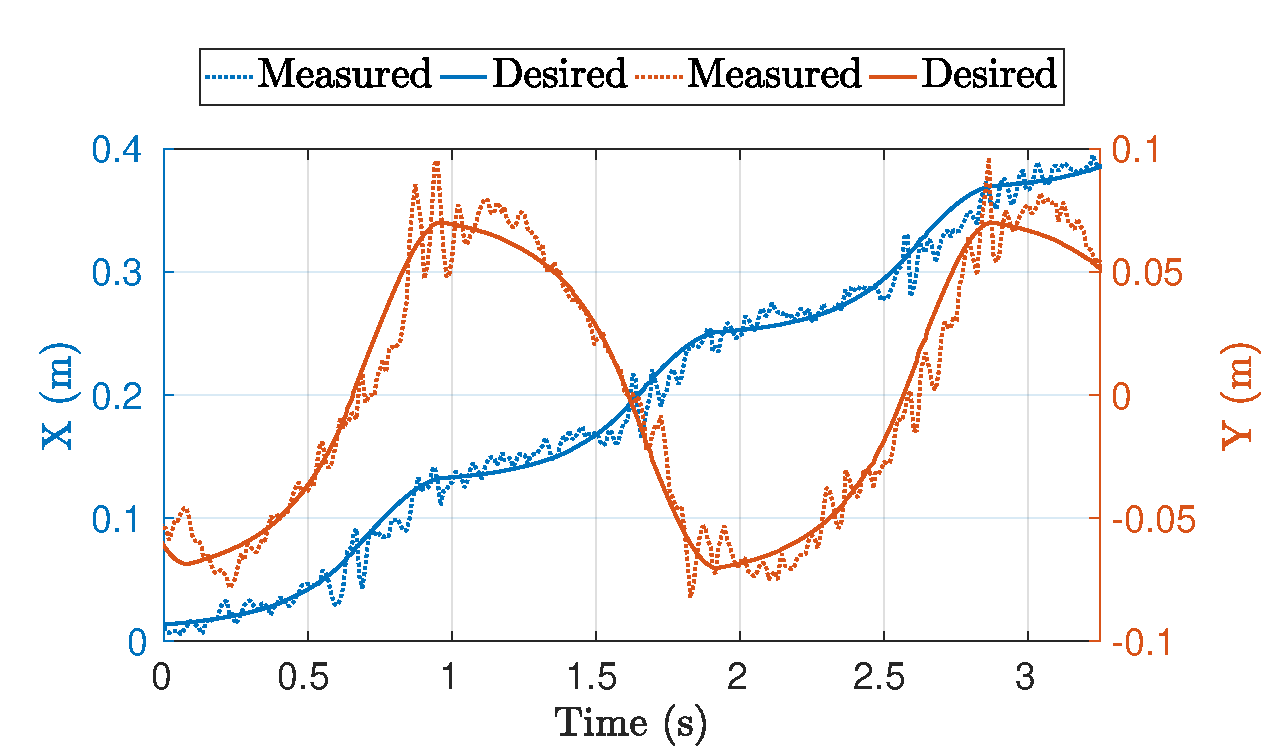
\includegraphics[width=\textwidth]{chapter_simplified_benchmarking/figures/inst_pos-min_vel-dcm.pdf}
        \caption{DCM}
        \label{fig:inst_pos-min_vel-dcm}
    \end{subfigure}
    \hfill
    \begin{subfigure}[b]{0.49\textwidth}
        \centering
        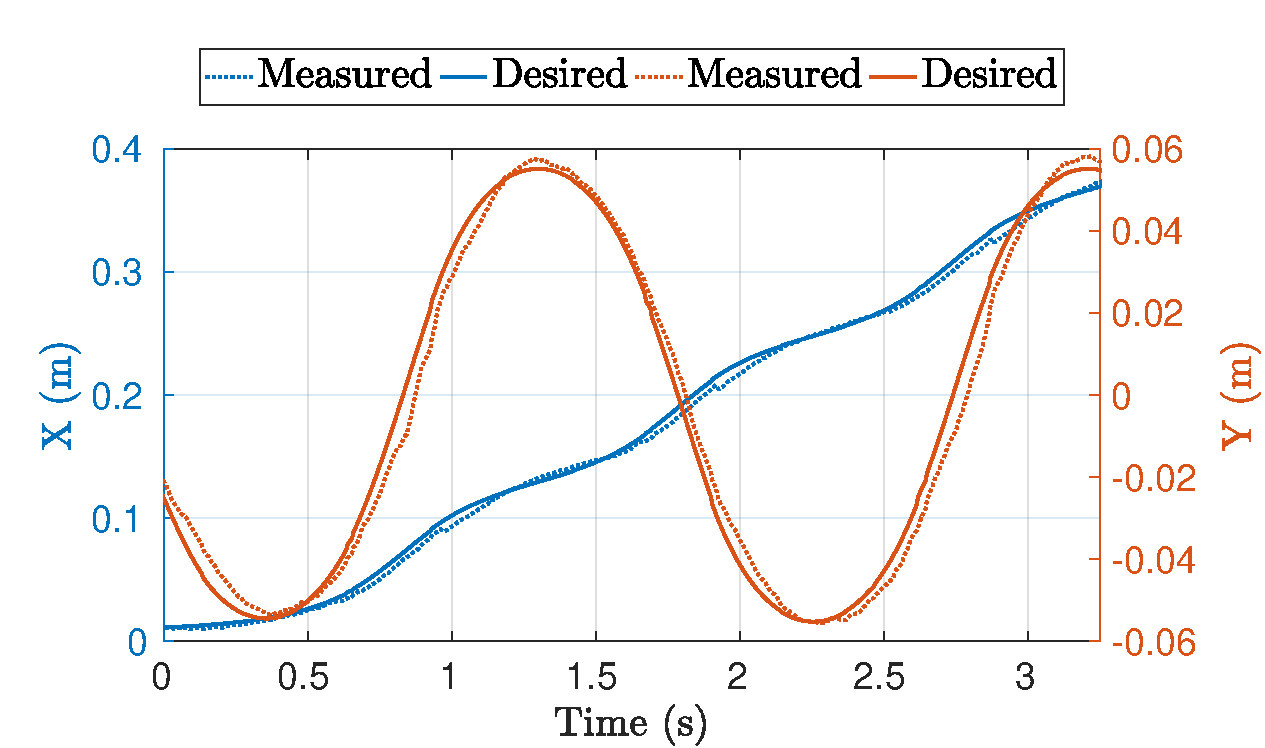
\includegraphics[width=\textwidth]{chapter_simplified_benchmarking/figures/inst_pos-min_vel-com.pdf}
        \caption{CoM}
        \label{fig:inst_pos-min_vel-com}
    \end{subfigure}
    \hfill
    \begin{subfigure}[b]{0.49\textwidth}
        \centering
        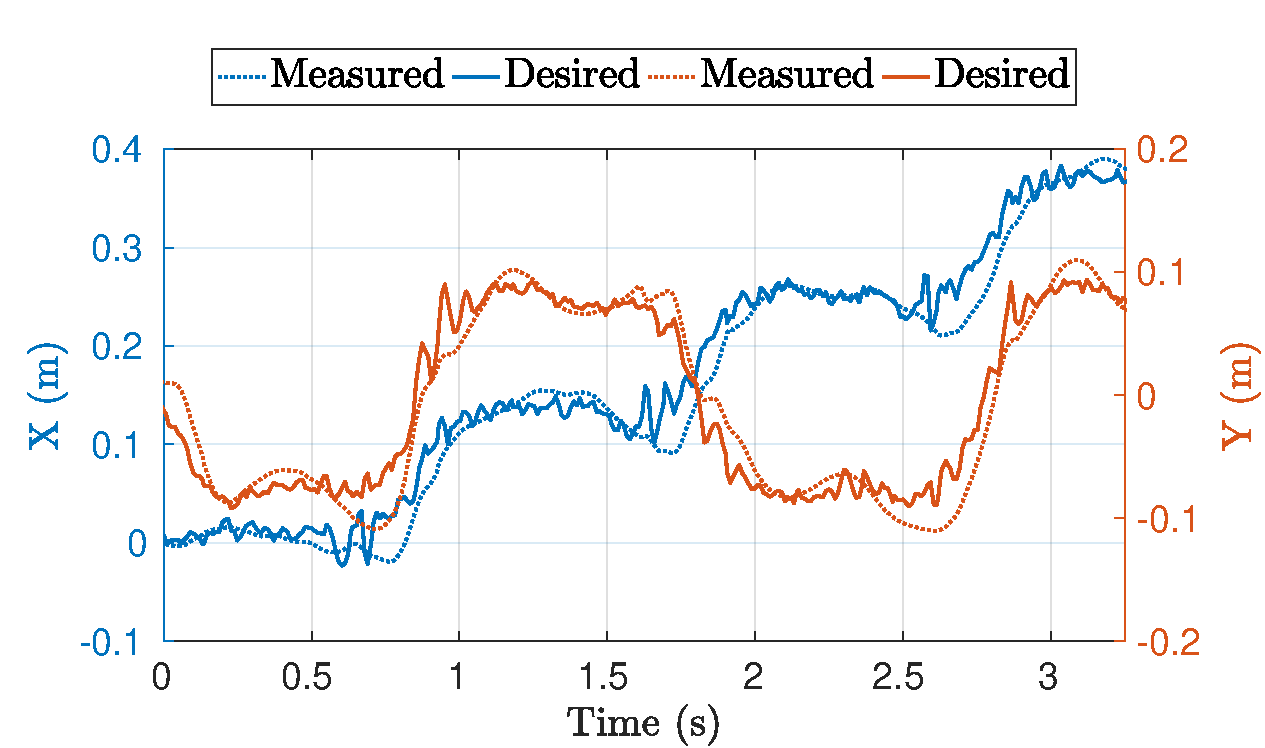
\includegraphics[width=\textwidth]{chapter_simplified_benchmarking/figures/inst_pos-min_vel-zmp.pdf}
        \caption{ZMP}
        \label{fig:inst_pos-min_vel-zmp}
    \end{subfigure}
    \end{myframe}
    \caption{Tracking of the DCM (a), CoM (b) and ZMP (c) using the instantaneous controller with the whole-body controller as position control. Walking velocity:  $\SI{0.19}{\meter \per \second}$.}
\end{figure}

\begin{figure}[t]
    \begin{myframe}{Predictive + Position Control}
     \centering
    \begin{subfigure}[b]{0.49\textwidth}
        \centering
        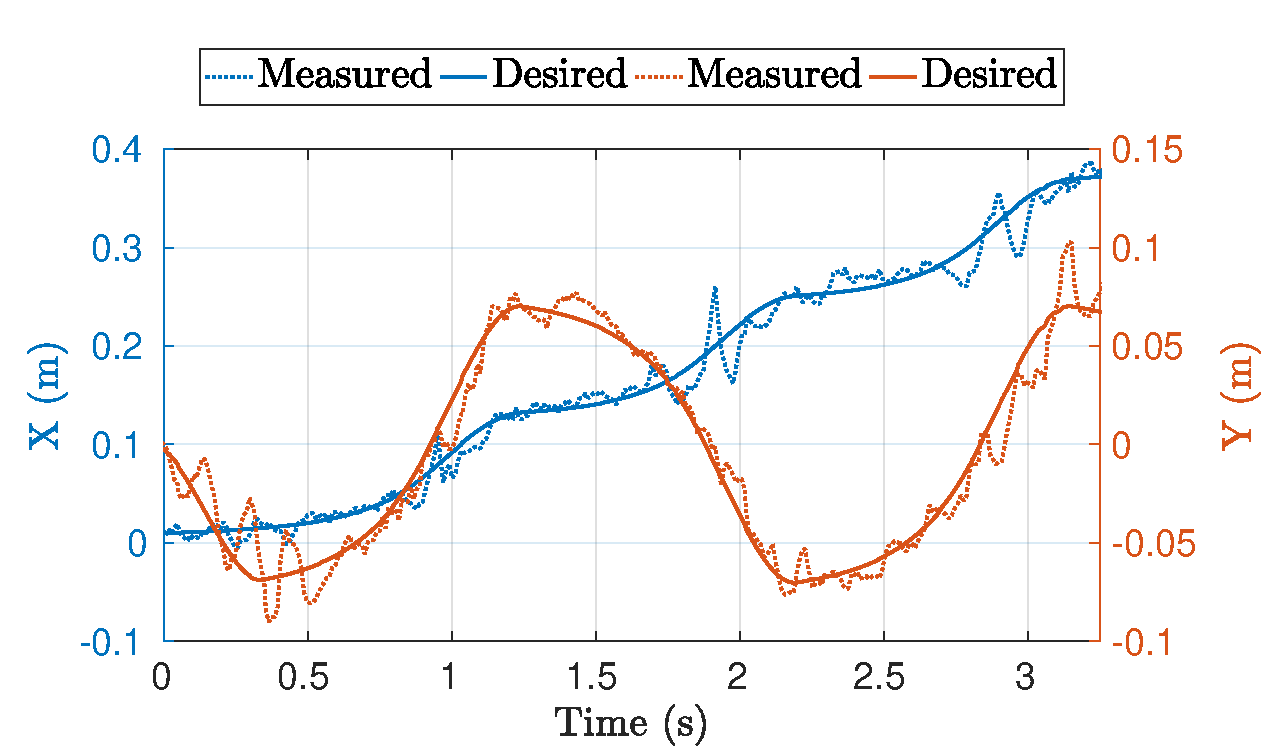
\includegraphics[width=\textwidth]{chapter_simplified_benchmarking/figures/mpc_pos-min_vel-dcm.pdf}
        \caption{DCM}
        \label{fig:mpc_pos-min_vel-dcm}
    \end{subfigure}
    \hfill
    \begin{subfigure}[b]{0.49\textwidth}
        \centering
        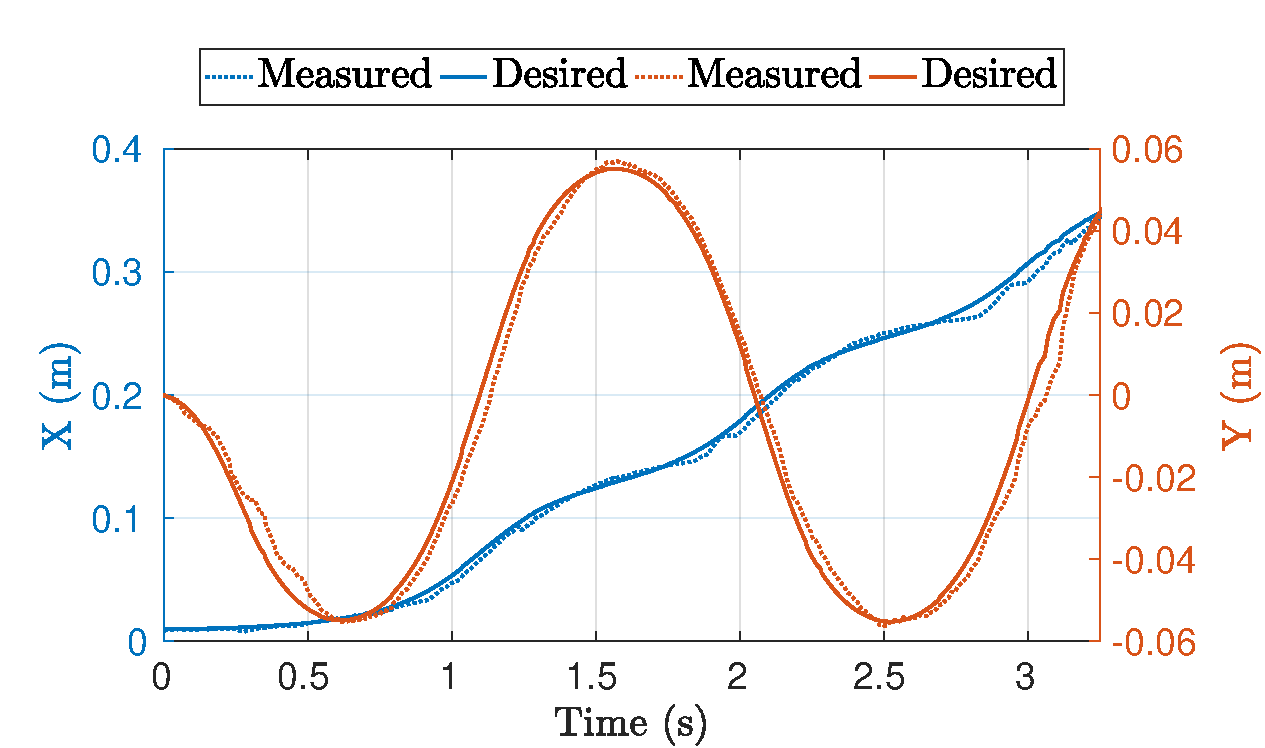
\includegraphics[width=\textwidth]{chapter_simplified_benchmarking/figures/mpc_pos-min_vel-com.pdf}
        \caption{CoM}
        \label{fig:mpc_pos-min_vel-com}
    \end{subfigure}
         \begin{subfigure}[b]{0.49\textwidth}
        \centering
        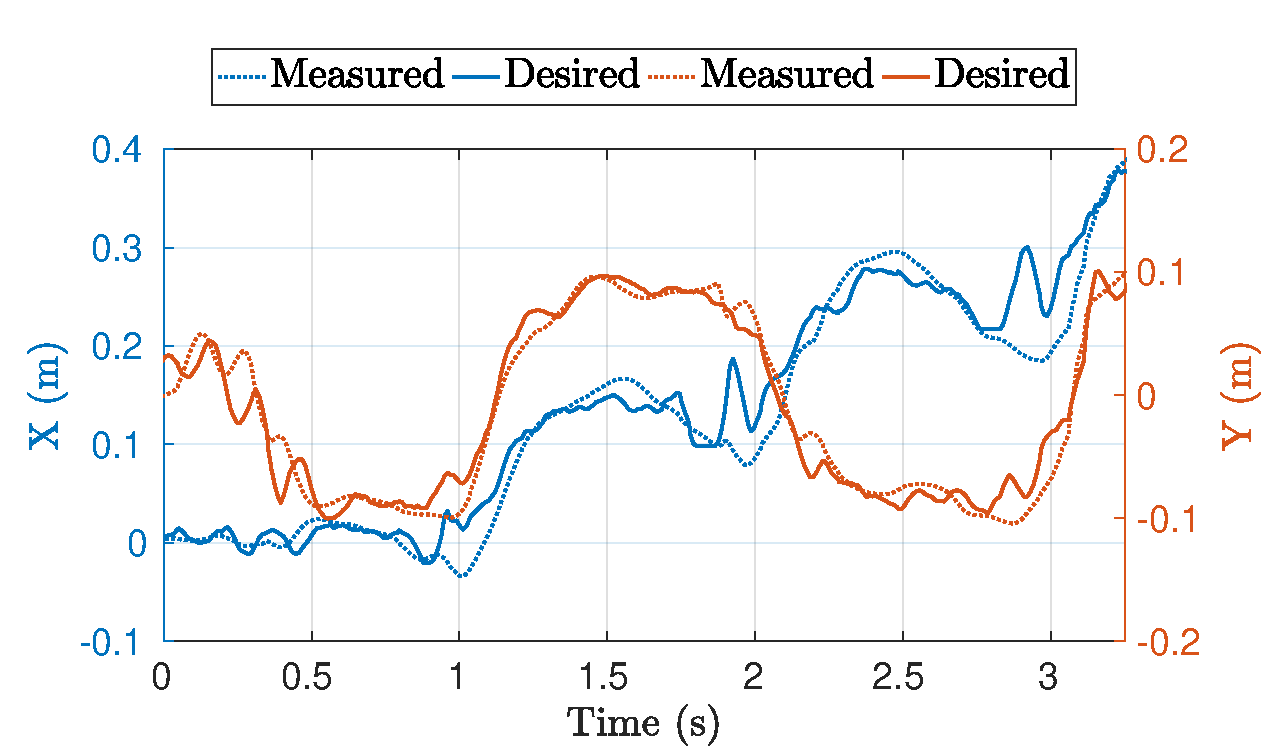
\includegraphics[width=\textwidth]{chapter_simplified_benchmarking/figures/mpc_pos-min_vel-zmp.pdf}
        \caption{ZMP}
        \label{fig:mpc_pos-min_vel-zmp}
    \end{subfigure}
    \end{myframe}
    \caption{Tracking of the  DCM (a), CoM (b) and ZMP (c) using the MPC and the whole-body controller as position control. Walking velocity:  $\SI{0.19}{\meter \per \second}$.}
\end{figure}
\begin{figure}[t]
     \vspace*{-0.1cm}
    \begin{myframe}{Instantaneous + Position Control}
    \centering
        \begin{subfigure}[b]{0.49\textwidth}
        \centering
        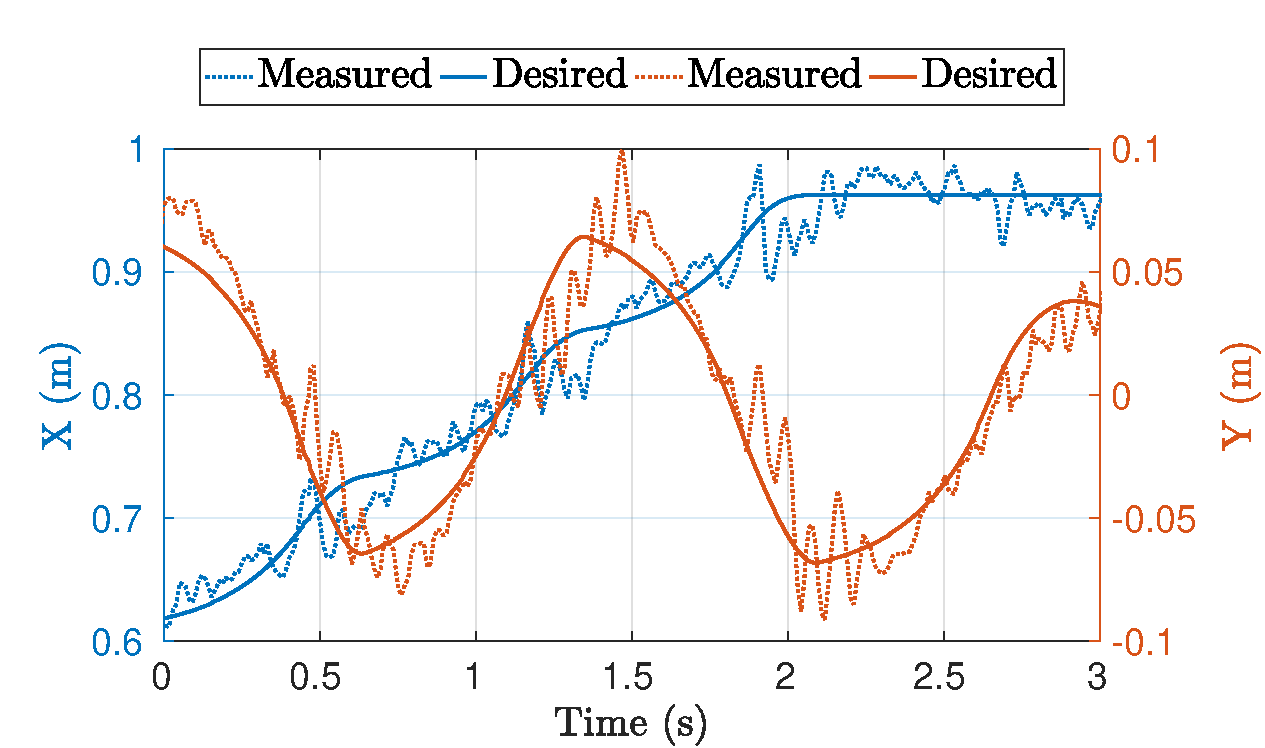
\includegraphics[width=\textwidth]{chapter_simplified_benchmarking/figures/inst_pos-max_vel-dcm.pdf}
        \caption{DCM}
        \label{fig:inst_pos-max_vel-dcm}
    \end{subfigure}
    \hfill
     \begin{subfigure}[b]{0.49\textwidth}
        \centering
        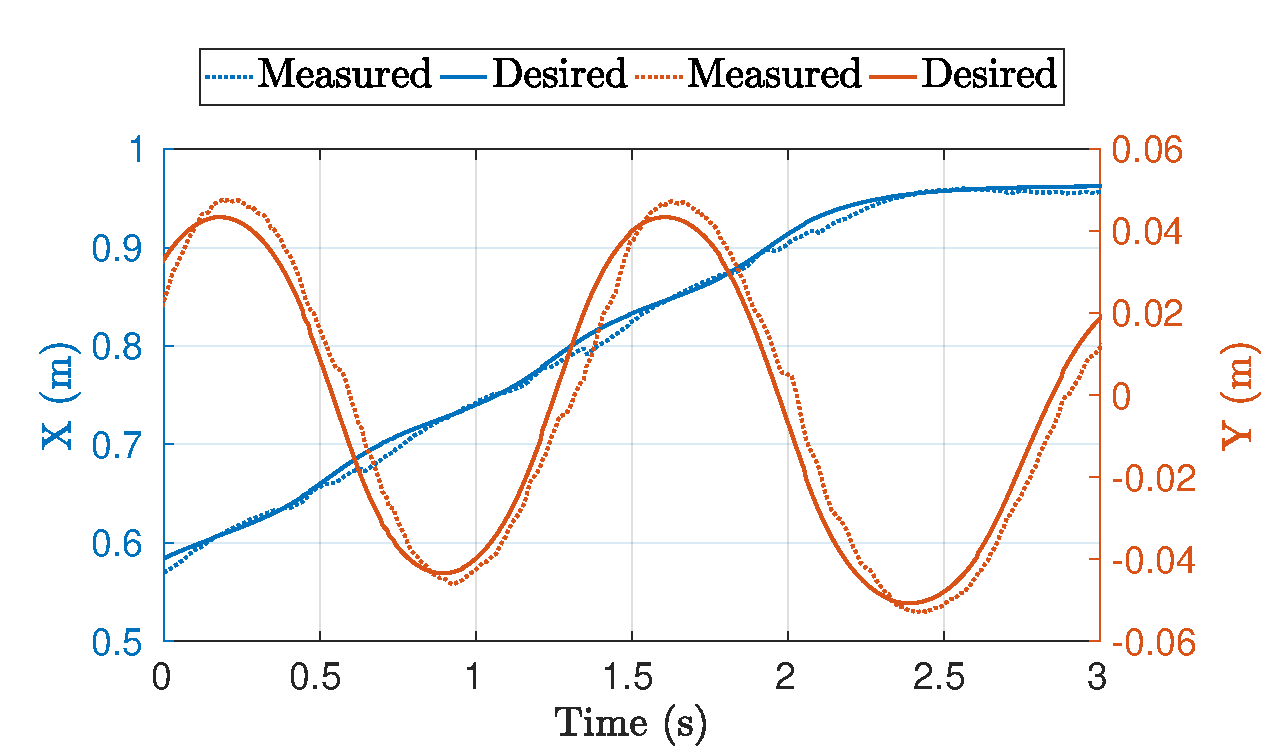
\includegraphics[width=\textwidth]{chapter_simplified_benchmarking/figures/inst_pos-max_vel-com.pdf}
        \caption{CoM}
        \label{fig:inst_pos-max_vel-com}
    \end{subfigure}
    \hfill
    \begin{subfigure}[b]{0.49\textwidth}
        \centering
        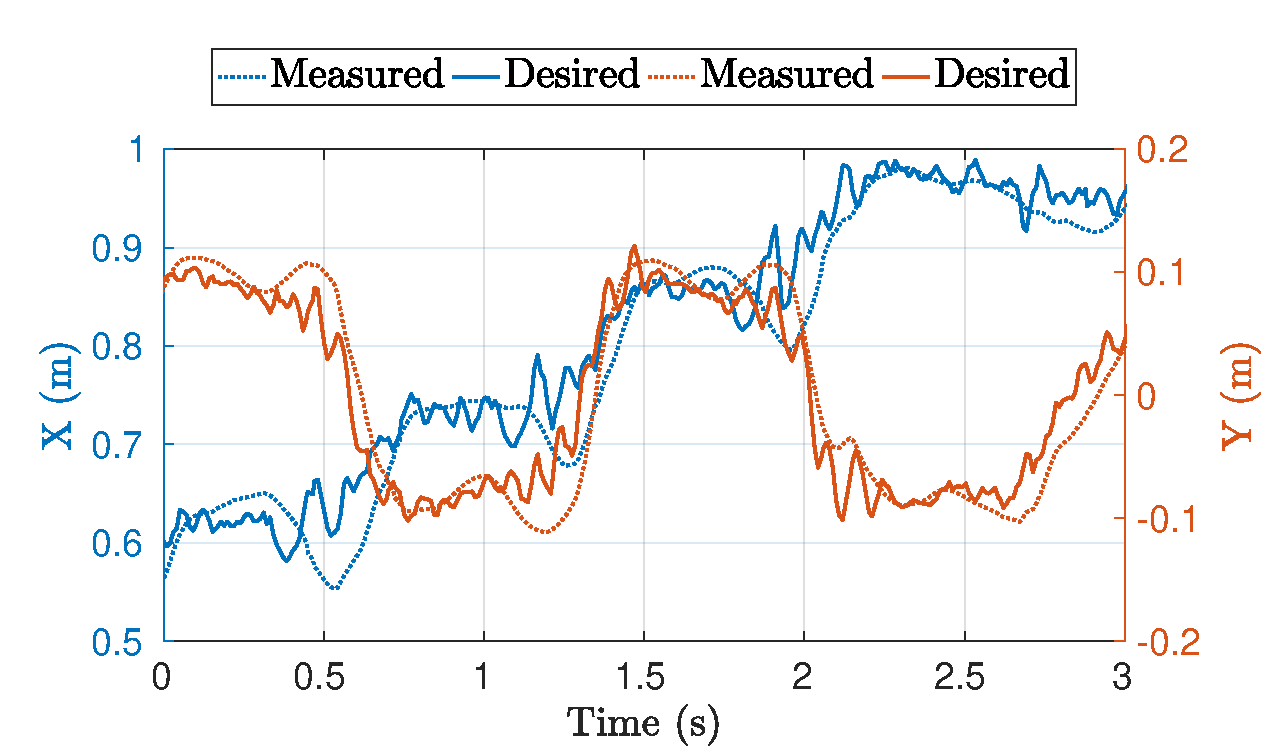
\includegraphics[width=\textwidth]{chapter_simplified_benchmarking/figures/inst_pos-max_vel-zmp.pdf}
        \caption{ZMP}
        \label{fig:inst_pos-max_vel-zmp}
    \end{subfigure}
    \end{myframe}
    \caption{Tracking of the DCM (a), CoM (b) and ZMP (c) with the instantaneous and whole-body QP control as position.  Walking velocity: $\SI{0.41}{\meter \per \second}$.}
\end{figure}
\begin{figure}[t]
    \begin{myframe}{Predictive + Position Control}
    \centering
    \begin{subfigure}[b]{0.49\textwidth}
        \centering
        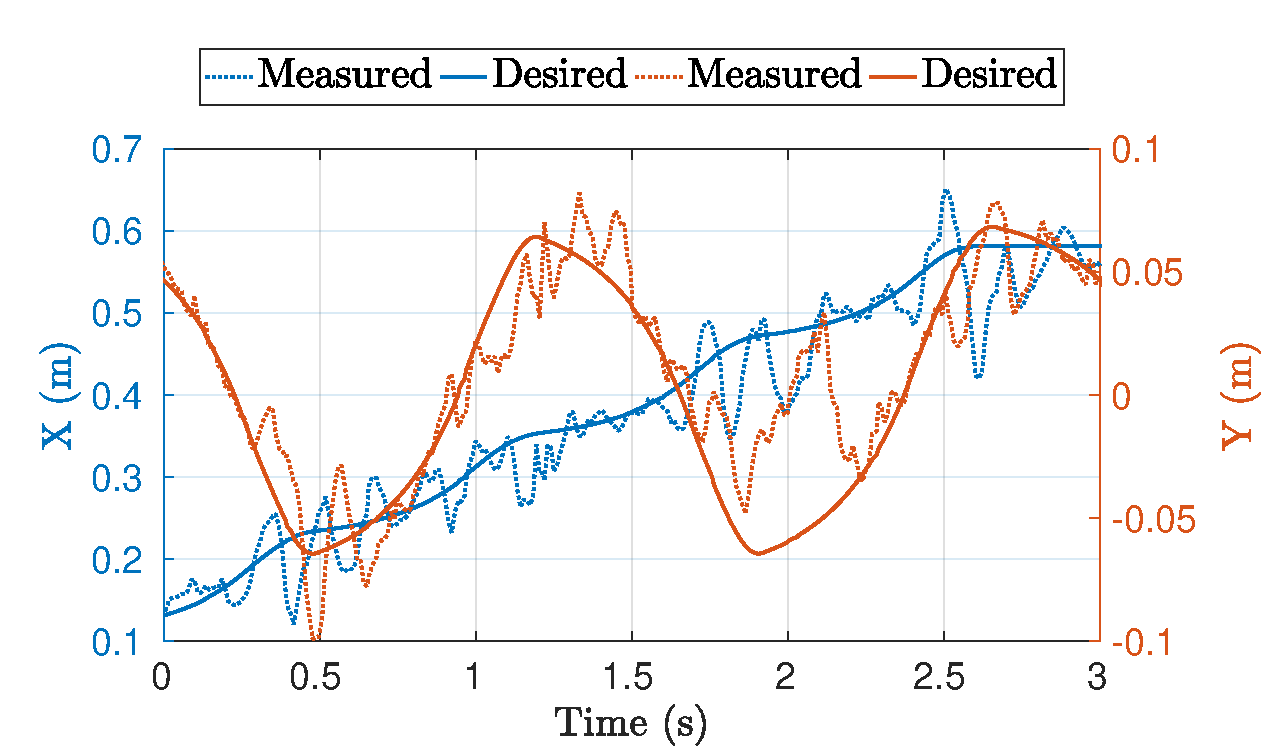
\includegraphics[width=\textwidth]{chapter_simplified_benchmarking/figures/mpc_pos-max_vel-dcm.pdf}
        \caption{DCM}
        \label{fig:mpc_pos-max_vel-dcm}
    \end{subfigure}
    \hfill
     \begin{subfigure}[b]{0.49\textwidth}
        \centering
        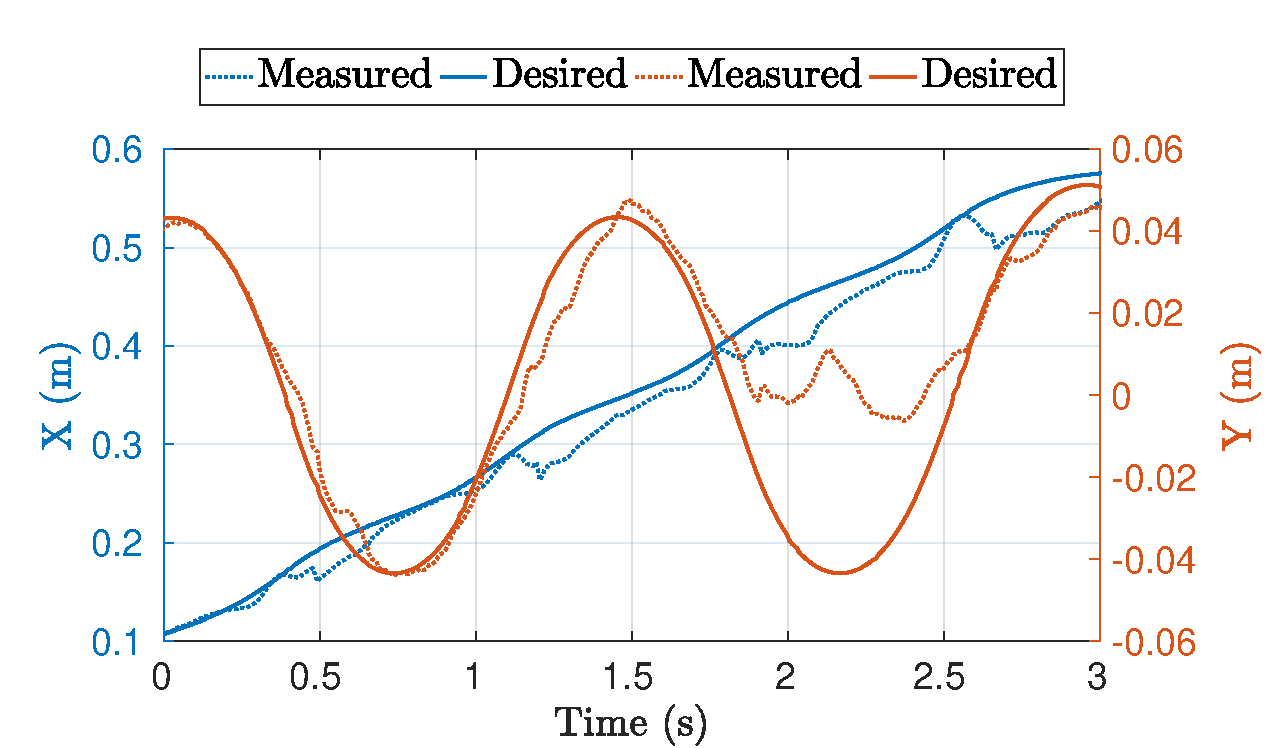
\includegraphics[width=\textwidth]{chapter_simplified_benchmarking/figures/mpc_pos-max_vel-com.pdf}
        \caption{CoM}
        \label{fig:mpc_pos-max_vel-com}
    \end{subfigure}
    \hfill
    \begin{subfigure}[b]{0.49\textwidth}
        \centering
        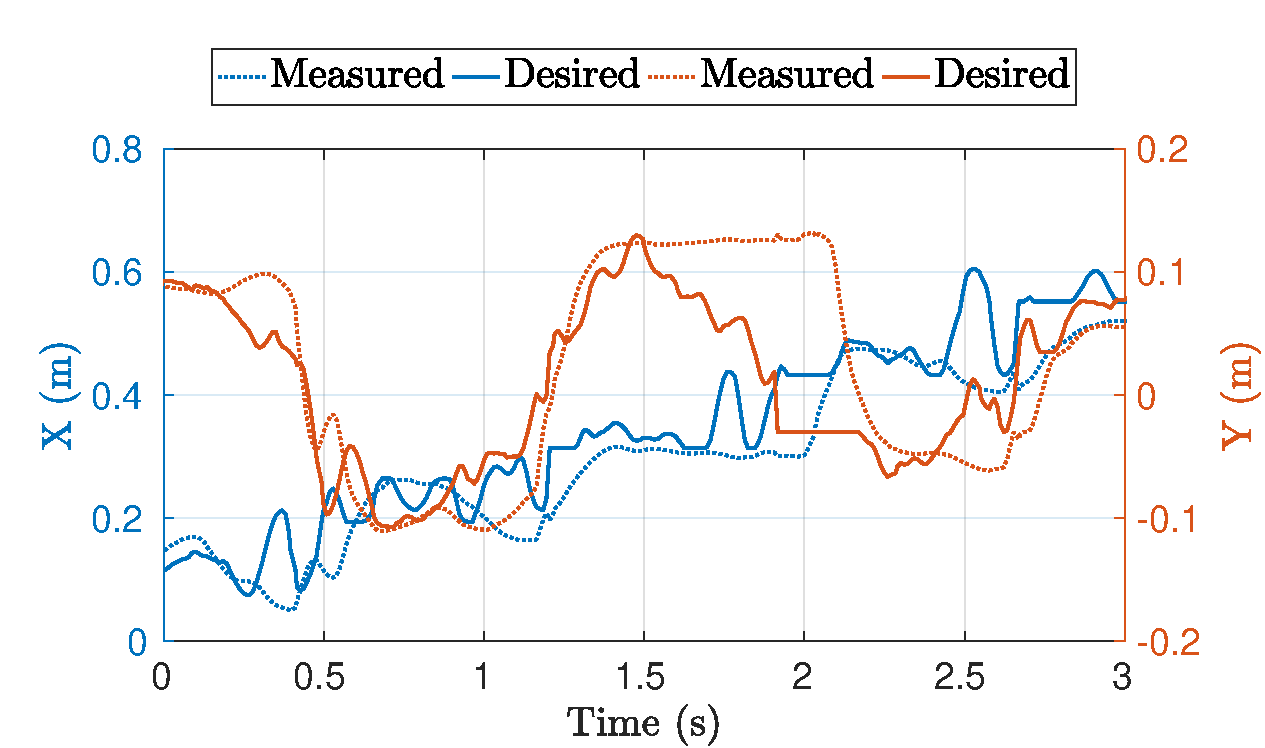
\includegraphics[width=\textwidth]{chapter_simplified_benchmarking/figures/mpc_pos-max_vel-zmp.pdf}
        \caption{ZMP}
        \label{fig:mpc_pos-max_vel-zmp}
    \end{subfigure}
    \end{myframe}
    \caption{Tracking of the  DCM (a), CoM (b) and ZMP (c) with the predictive and whole-body QP control as position control. At $t\approx \SI{2}{\second}$, the robot falls down.  Walking velocity: $\SI{0.41}{\meter \per \second}$.}
    \vskip-0.5cm
\end{figure}

We compare the control laws~\eqref{eq:reactive_dcm} and~\eqref{eq:mpc_solution_simplified}, which both generate a (desired) center of pressure that attempts to stabilize the desired DCM. To simplify the comparison, the controller of the \emph{whole-body QP layer} is kept fixed in this section, and we show and discuss only the results when the robot is position controlled. A complete comparison of the kinematics-based whole-body controllers is presented in Section~\ref{sec:wbc_experimental_results}.
In the following experiments, we set the time horizon of the predictive control to $\SI{2}{\second}$.

\subsection{Experiment 1: a forward robot speed of 0.1563 m s$^{\text{-1}}$}
Figures \ref{fig:inst_pos-min_vel-dcm} and \ref{fig:mpc_pos-min_vel-dcm} show the DCM tracking performances obtained with the instantaneous and predictive controllers, respectively. Both controllers seem to show good tracking performances, and the DCM error is kept below $\SI{5}{\centi \meter}$ in both cases. Note, however, that the instantaneous controller induces faster variations of the measured DCM. This contributes to the overall higher vibrations of the robot. One of the reasons for this variation is that the instantaneous controller~\eqref{eq:reactive_dcm} injects a (desired) center of pressure proportional to the measured DCM, which in turn contains the center of mass velocity. To mitigate this, we may filter the joint velocities appropriately. However, in our case, the joint velocities were not filtered to avoid delays in the measured DCM. Our experience showed that adding a filter to joint velocities is not an easy task, and we did not find the right trade-off for obtaining overall performance improvements. 

Figures~\ref{fig:inst_pos-min_vel-com} and \ref{fig:mpc_pos-min_vel-com} present CoM tracking performances, which are mainly dependent on the ZMP-CoM controller~\eqref{eq:ZMP_controller}. This controller receives the desired DCM values from the \emph{simplified model control} layer, which are obtained with the instantaneous or predictive controllers. In both cases, the CoM error is kept below $\SI{2}{\centi \meter}$. Figures~\ref{fig:inst_pos-min_vel-zmp} and~\ref{fig:mpc_pos-min_vel-zmp} represent the ZMP tracking performance, which is still mainly dependent on the ZMP-CoM controller~\eqref{eq:ZMP_controller}. It is important to note that the desired ZMP is smoother when the \emph{simplified model control} uses the predictive law~\eqref{eq:mpc_solution_simplified} to generate it. Indeed, this is a tunable property that depends on the associated weight in the cost function of the MPC problem. Although this smoother behavior contributes to less robot vibrations, overall robot performance became less reactive and, consequently, less robust to robot falls. Although the extensive hand-made tuning, we were not able to increase the robot velocity when the \emph{simplified model control} used the predictive law~\eqref{eq:mpc_solution_simplified}. 

\subsection{Experiment 2: a forward robot speed of 0.3372 m s$^{\text{-1}}$}
At a robot's desired walking speed of $\SI{0.3372}{\meter \per \second}$, there is initially no significant difference between the DCM tracking obtained with instantaneous and predictive control laws -- see Figures~\ref{fig:mpc_pos-max_vel-dcm} and~\ref{fig:inst_pos-max_vel-dcm} for $t < \SI{1.5}{\second}$. However, fast robot walking velocities require fast variations of the desired CoM and ZMP. This fast variation degrades the performance of the predictive controller around $t = \SI{1.5}{\second}$ -- see Figure~\ref{fig:mpc_pos-max_vel-zmp}. Clearly, these bad performances, in turn, induce poor tracking of the DCM shown in Figure~\ref{fig:mpc_pos-max_vel-dcm} at $t\approx \SI{2}{\second}$, and consequently the robot falls. At this point, one is tempted to increase the gain $K_\text{ZMP}$ of the controller~\eqref{eq:ZMP_controller}, which shall induce a better tracking of the ZMP. Unfortunately, this leads to higher robot oscillations induced by the noise on the estimated ZMP. And, as a consequence, the robot falls. 

We can conclude that the \emph{predictive simplified control} is much less robust than the \emph{instantaneous simplified control} with respect to ZMP tracking errors. Adding a low-pass filter to the ZMP measurement may improve the overall performance. However, in our case, adding filters led to slower system response and, consequently, to the robot falling.



\section{Conclusions \label{sec:conclusions_flexible_joint}}
This chapter presents the design of a whole-body QP control layer for a humanoid robot affected by link flexibility. We model the flexibility by introducing equivalent passive joints that simulate the motion caused by the link deformation.
We then considered the passive joints position and velocity as state of the floating base system dynamics. Thanks to this choice, we develop a whole-body controller that implicitly considers the joint flexibility in the stabilization problem. 
The chapter also details the design of an estimator that aims at computing the flexible joint state in real-time. 
\par
The proposed approach is validated in a simulated version of the TALOS humanoid robot, where its hip flexibility has a significant impact while performing locomotion tasks. Moreover, the architecture is then compared with a whole-body controller that considers all links of the robot rigid.
\par
As a future work, we plan to mitigate the discontinuity of the contact forces by performing a smother transition between contiguous support phases. We also plan to make a detailed comparison with other state-of-the-art controllers that
consider the flexibility of the robot link~\citep{Villa2022TorqueFlexibility}. In addition, we plan to validate the architecture on the real robot.




